\section{Related Work}
\label{sec:related}

\subsection{Sampling Algorithms}
Rather than count the frequency of each packet, one family of heavy hitter algorithms is based on infrequent sampling. While this approach improves scalability and drastically reduces memory usage, sampling comes at the cost of decreased accuracy. The algorithms Sampled NetFlow~\cite{netflow} and Sample and Hold~\cite{samplehold} follow this approach by sampling each packet with some very small probability, such as 0.1 percent or even 0.01 percent. Sample and Hold improves upon Netflow, since once a flow is sampled, a corresponding counter is held in a hash table in flow memory until the end of the measurement interval. The entry for a flow is updated for every subsequent packet belonging to the flow. According to this scheme, the error is proportional to $1/M$, as opposed to $1/M$ for a classical sampling algorithm, where M is the available memory. 

\subsection{Sketch Algorithms}
Sketch algorithms are a family of algorithms that attempt to answer questions about data streams by leveraging approximation. By sacrificing accuracy, sketch algorithms allow the heavy hitter problem to be tackled using a limited amount of memory. One of the most prominent of these algorithms is Count-Min Sketch~\cite{countmin}, which uses a two-dimensional hash table to approximate counts. Each packet is hashed using d different hash functions, and the counter in each of the d corresponding buckets is incremented. Hash collisions will cause certain bucket counts to be incremented for different flow identifiers, so to approximate the count for a given identifier, it is hashed using the d hash functions, and the minimum of these bucket counts it used. This method is hardware-friendly, but sketch based algorithms do not track the flow identifiers associated with each count, so reporting the frequency of the top k flows is not accurate.

\subsection{Counter Based Algorithms}
Counter Based Algorithms process every flow, but due to memory constraints, are only able to maintain a counter of a constant number of the heaviest flows. Therefore, these algorithms aim to retain counters of only heavy hitters while ignoring lighter flows through the use of strategic admission and eviction policies. Space Saving~\cite{spacesaving} maintains a table of the frequencies of N flows, evicting the least frequent flow each time an unmonitored flow is encountered. The newly admitted element assumes the frequency of the evicted flow. This eviction policy results in large errors for heavy-tailed workloads, where many new small flows may wrongly evict larger flows. Furthermore, depending on the hardware implementation, it may be resource intensive to find the least frequent flow in the table for every newly encountered flow. 

The intuition behind Randomized Admission Policy (RAP)~\cite{rap} is to minimize this error by being much more conservative about the elements that are admitted into the table. Instead of evicting the minimum element in the table for every new flow encountered, RAP only admits new flows with a probability of $1/(c_m + 1)$, where $c_m$ is the minimal counter value. By being more conservative, RAP has increased accuracy over Space Saver, but also makes it more difficult for new larger flows to gain admission. In our approach, we adopt elements of the randomized admission policy to prevent false evictions while also dampening the adverse effects of a conservative policy. 

\begin{figure}[t]
  \centering
    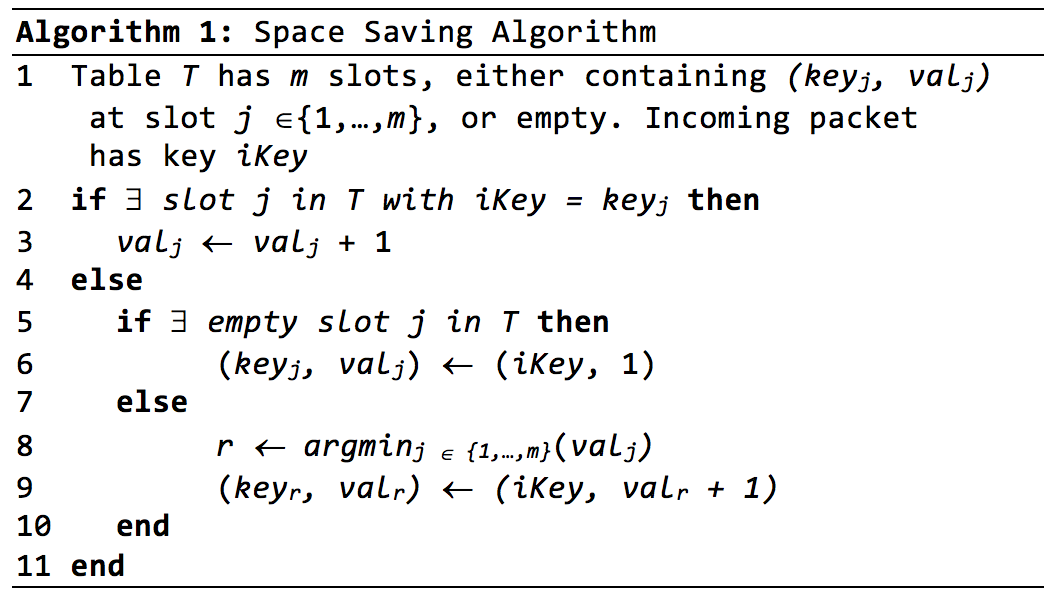
\includegraphics[scale=0.5]{alg1}
     \label{fig:bp-image}
\end{figure}

HashPipe~\cite{hashpipe} is heavily inspired by Space Saver, but leverages feed-forward packet processing to divide the task of finding the minimum into small parts. The algorithm consists of d stages, each with its own hash function hd and an associated hash table. When a packet enters the pipeline at the first stage, the hash function h0 is used to hash its identifier to a bucket. Each bucket will contain a flow identifier and its associated count. If the identifier of an incoming packet matches the identifier stored in the bucket it hashes to, the count is incremented, and no further processing is done. Similarly, if the bucket is empty, the identifier is added with a count of 1, and processing stops. However, the rest of the pipeline comes into play if the incoming packet identifier does not match the stored packet identifier. In this case, the stored packet will be evicted, and the incoming packet will be stored in its place with a count of 1. In actual implementations of HashPipe on hardware, the identifier and count of the ``evicted'' packet is added to the incoming packet as metadata, and the original packet continues to flow down the pipeline with this metadata.

\begin{figure}[t]
  \centering
    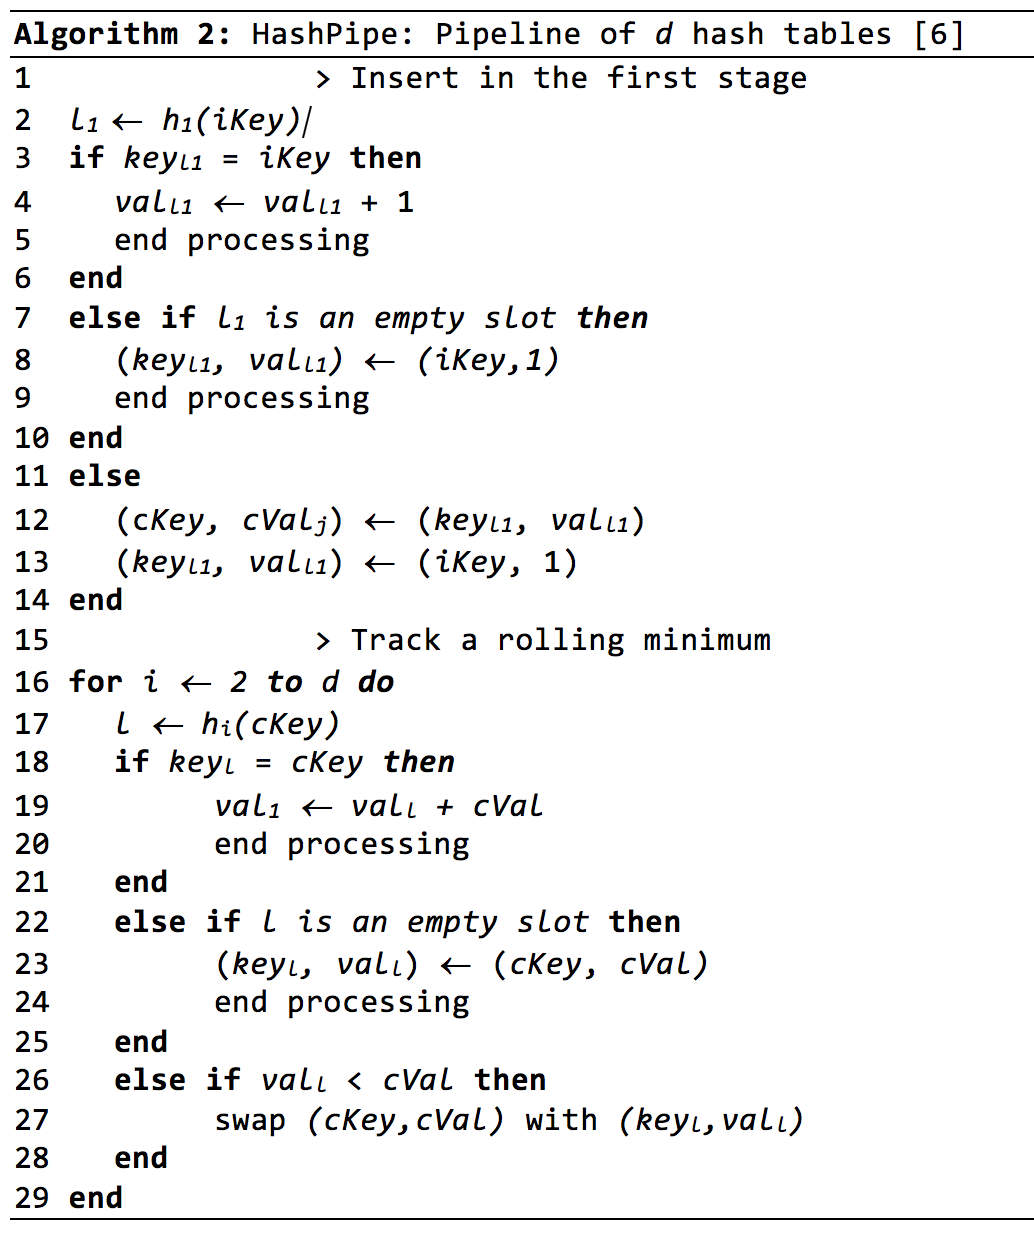
\includegraphics[scale=0.42]{alg2}
     \label{fig:bp-image}
\end{figure}

In subsequent stages, the key-counter pair that has been evicted is hashed using the corresponding hash function hd and it is compared to the stored value in that bucket. Instead of always evicting like in the first stage, the stored value will only be evicted if it is the minimum between the two counter values. If the stored value is less, the key-counter pairs are swapped, and the key previously in the table becomes the carried key. This same process is repeated at each stage until one pseudo-minimum value is carried off the end.

Instead of attempting to find a true minimum, as is the case in Space Saver, HashPipe settles for a probabilistic minimum, obtained by comparing only one value per stage. The main idea behind the pipeline is that heavy flows will be retained and lighter flows will be evicted over time. HashPipe is useful because for each packet, there is only one read per table. This allows for efficient stream processing and gets around hardware constraints that do not allow multiple reads to the same table. The downside of this scheme is that it does not prevent duplicate keys across different tables. When a count is stored for the same keys in different stages, this reduces the space available to hold onto heavier flows. However, duplicates have been shown to account for only 5-10 percent of table space, and have a limited impact on accuracy~\cite{hashpipe}. With a fixed amount of memory available to the hardware, the number of stages d can be tuned: a greater number of stages increases heavy flow retention because more slots are sampled to pick a minimum, but it will increase the number of duplicates.